\documentclass[11pt]{article}
\usepackage[margin=1in]{geometry}
\usepackage{xcolor,mdframed,amsmath,amssymb,booktabs,graphicx,float,hyperref}
\usepackage[T1]{fontenc}
\hypersetup{colorlinks=true,linkcolor=blue,urlcolor=blue}
\setlength{\parindent}{0pt}
\setlength{\parskip}{5pt}
\setlength{\textfloatsep}{10pt}
\setlength{\intextsep}{9pt}
\renewcommand{\arraystretch}{1.15}
\begin{document}
\noindent\rule{\linewidth}{2pt}
{\large\textbf{Srikar Palani, Suprathik Vinayakula}}\hfill\textbf{CS 598: Midterm Project}\\
\href{mailto:palani3@illinois.edu}{palani3@illinois.edu},
\href{mailto:sv53@illinois.edu}{sv53@illinois.edu}\hfill Fall 2026\\[-3pt]
\noindent\rule{\linewidth}{2pt}
\begin{center}
{\Large\bfseries Parallel implicit heat diffusion}\\[3pt]
{\large Jacobi versus conjugate gradient}
\end{center}
\section{Project overview}

This project asks how much a parallel solver benefits from additional processors, and when communication becomes its main cost. We compare Jacobi and conjugate gradient (CG) on the same heat-diffusion problem using MPI on the Illinois Campus Cluster. The comparison focuses on \textbf{time to reach an equally accurate solution}, rather than how quickly either method performs one iteration.

The main finding is that CG was faster at every tested strong-scaling configuration. However, adding more processes eventually gives diminishing returns. On the smaller grid, both methods reached their best sampled runtime at 32 processes and became slower at 48 and 64. The larger grid continued to benefit through 64 processes, even after MPI accounted for more than half of the measured computation-plus-communication time.

\section{The physical problem and the two solvers}

Imagine a square plate with two warm regions inside and all four edges held at zero temperature. Heat spreads across the plate and escapes through its edges. We represent the interior by an N-by-N grid. A larger N gives a more detailed representation of the same plate.

We advance the temperature with backward Euler. This implicit method requires solving a linear system at each physical time step:

\[
A\,T^{n+1}=T^n
\]

Here, the right-hand side is the current temperature field and the unknown is the next field. The action of A involves only a grid point and its four immediate neighbors. The program applies this five-point stencil directly, so it does not store a large dense matrix.

\begin{table}[H]
\centering\small
\begin{tabular}{lll}
\toprule
Method & How it progresses & Main tradeoff \\
\midrule
Jacobi & Repeated local corrections & Simple updates, many iterations \\
CG & A sequence of search directions & Fewer iterations, more synchronization \\
\bottomrule
\end{tabular}
\caption{Both methods solve the same linear system. CG uses no preconditioner.}
\end{table}

A \textbf{physical time step} advances the heat simulation. A \textbf{solver iteration} is one update toward solving the system within that step. These are different quantities: five physical steps can require hundreds of solver iterations.

\clearpage

\section{How the work is distributed}

MPI divides the grid into rectangular blocks, one per process, also called a rank. Each rank updates its own temperatures. Along a block edge, it first obtains neighboring values from the adjacent rank. These exchanged border values are called \textbf{halos}. The partition also supports uneven block sizes.

Halo exchanges involve neighboring ranks. Global reductions combine values from every rank to calculate a dot product or check convergence. CG performs two dot products per iteration. Jacobi checks convergence after the first update, every ten updates, and at its iteration limit. Both start each solve from the previous temperature field.

\section{Correctness and experimental method}

\textbf{Accuracy comes before timing.} Both solvers use a relative-residual tolerance of 10$^{-8}$. The residual measures how well the computed field satisfies the system. An independent check after every solve rejects inaccurate results, even when the solver internally reports convergence.

The stored cluster tests passed comparisons with an independent serial solver, an analytic sine solution, and a refinement study. They also cover uneven blocks, boundaries, zero input, and failure cases. Separate diagnostics verified timing selection and a CG case with a misleading internal residual. Performance runs exclude this extra instrumentation.

\begin{table}[H]
\centering\small
\begin{tabular}{ll}
\toprule
Experimental choice & Setting \\
\midrule
Compute resources & Two exclusive AMD EPYC 7713 nodes \\
Process placement & One node at P = 1; both nodes at P >= 2 \\
Strong-scaling grids & N = 512 and 1024 \\
Strong-scaling processes & P = 1, 2, 4, 8, 16, 24, 32, 48, 64 \\
Measured work & Five physical steps after a reset warm-up \\
Repetitions & Five trials per configuration \\
\bottomrule
\end{tabular}
\caption{The extended study contains 280 valid runs across 56 configurations.}
\end{table}

Ranks were bound to physical cores. We report the median of five trials. Each trial sums the slowest-rank time for each of five steps, since all ranks must finish. Every timing component comes from that same rank within a step. The timer includes solver work and MPI calls, but excludes field initialization, final accuracy checks, and output.

All 280 runs completed five steps and passed the tolerance; the largest residual was 9.985 $\times$ 10$^{-9}$. Earlier experiments remain separate from this dataset.

\clearpage

\section{Results and interpretation}

\subsection{Strong scaling: solve the same problem faster}

\textbf{Strong scaling keeps the total grid fixed and adds processes.} Each process owns a smaller block. Ideally, doubling the process count halves runtime. We express speedup as the one-process runtime divided by the P-process runtime:

\[
\mathrm{Speedup}(P)=\frac{T_1}{T_P},\qquad \mathrm{Efficiency}(P)=\frac{\mathrm{Speedup}(P)}{P}
\]

\begin{figure}[H]
\centering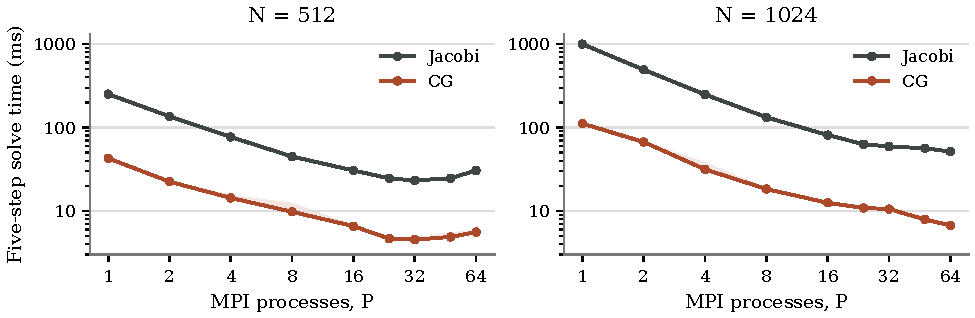
\includegraphics[width=\linewidth]{figures/strong_runtime.pdf}
\caption{Strong scaling for both grids. Each point is the median of five trials; shading shows the minimum-to-maximum trial range. Both axes use logarithmic spacing.}
\end{figure}

\begin{table}[H]
\centering\small
\begin{tabular}{lrrrr}
\toprule
P & N=512 Jacobi & N=512 CG & N=1024 Jacobi & N=1024 CG \\
\midrule
1 & 251.074 & 42.735 & 998.070 & 111.365 \\
8 & 44.845 & 9.755 & 132.570 & 18.296 \\
16 & 30.510 & 6.563 & 81.018 & 12.501 \\
32 & 23.190 & 4.525 & 59.066 & 10.525 \\
64 & 30.533 & 5.580 & 51.396 & 6.689 \\
\bottomrule
\end{tabular}
\caption{Selected median five-step solve times in milliseconds. All nine process counts appear in Figure 1.}
\end{table}

CG was faster in all 18 strong-scaling comparisons. At N = 512 and P = 32, CG took 4.525 ms versus 23.190 ms for Jacobi, a 5.13-fold advantage. At N = 1024 and P = 64, the corresponding times were 6.689 ms and 51.396 ms, a 7.68-fold advantage. These ratios compare medians from separate trials.

CG achieves this by requiring far fewer updates. For N = 1024, the five steps require 24 CG updates versus 450 Jacobi updates. A CG update is more expensive, but the smaller update count more than compensates. Relative speedup alone can hide this distinction: at 64 processes, Jacobi has a 19.42-fold speedup over its own baseline and CG a 16.65-fold speedup, yet CG still has the much lower absolute runtime.

\clearpage

\subsection{When communication becomes the larger cost}

As a fixed grid is split among more processes, each rank has less local work. It still exchanges halos and participates in global reductions. To describe that balance, we measure the MPI share as halo-plus-reduction time divided by computation-plus-MPI time. Other bookkeeping is excluded from this fraction. \textbf{MPI time includes waiting and imbalance}, so this is not a direct measurement of network-transfer time.

\begin{figure}[H]
\centering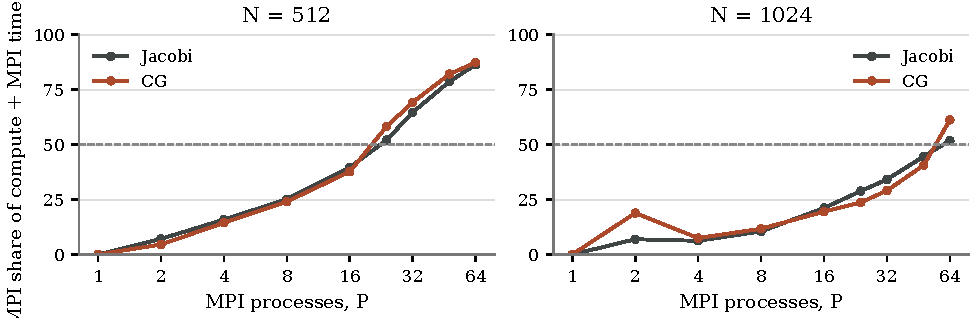
\includegraphics[width=\linewidth]{figures/communication_share.pdf}
\caption{The dashed line marks 50\% MPI time. Larger grids postpone the point at which MPI becomes the majority of the measured computation-plus-communication time.}
\end{figure}

For N = 512, both solvers cross 50\% between 16 and 24 processes. For N = 1024, both cross between 48 and 64. These are brackets between sampled configurations, rather than exact thresholds. At N = 1024 and P = 64, the median MPI shares are 51.8\% for Jacobi and 61.2\% for CG.

Communication dominance does not immediately imply worse runtime. The smaller grid becomes slower beyond 32 processes, while the larger grid still improves through 64. The larger grid retains enough local work for the additional processes to remain useful.

\subsection{Weak scaling: handle a larger problem in similar time}

\textbf{Weak scaling grows the grid along with the process count}, keeping the number of owned cells per process constant. Here, every process owns 256-by-256 cells. Ideal weak scaling would keep runtime constant as the total problem grows.

\begin{table}[H]
\centering\small
\begin{tabular}{lrrr}
\toprule
P & Total grid & Jacobi (ms) & CG (ms) \\
\midrule
1 & 256 x 256 & 69.737 & 15.431 \\
4 & 512 x 512 & 77.016 & 14.494 \\
16 & 1024 x 1024 & 81.397 & 12.608 \\
64 & 2048 x 2048 & 115.667 & 22.599 \\
\bottomrule
\end{tabular}
\caption{Weak scaling with 256-by-256 cells per process. Times cover five physical steps.}
\end{table}

From 1 to 64 processes, Jacobi grows from 69.7 to 115.7 ms and CG from 15.4 to 22.6 ms. Iteration counts also fall as the grid grows, partly masking the higher cost of each update. Average solve time per update rises from 0.127 to 0.289 ms for Jacobi and from 0.262 to 1.027 ms for CG. This ratio includes solver checks and setup within the timed solve; it is not a measurement of the update kernel alone.

\clearpage

\subsection{Larger timesteps increase the work per solve}

We use a timestep parameter r. With diffusivity fixed at 1, r is the physical timestep divided by the squared grid spacing. At a fixed grid, larger r advances the simulation farther per step and changes the linear system. The scaling studies use r = 2; here we vary it.

\begin{table}[H]
\centering\small
\begin{tabular}{lrrrr}
\toprule
r & Jacobi (ms) & CG (ms) & Jacobi updates & CG updates \\
\midrule
0.5 & 30.675 & 8.060 & 150 & 11 \\
2 & 81.935 & 12.983 & 450 & 24 \\
8 & 317.589 & 33.782 & 1920 & 85 \\
\bottomrule
\end{tabular}
\caption{Timestep sensitivity at N = 1024 and P = 16. Times and update counts cover five physical steps.}
\end{table}

From r = 0.5 to 8, Jacobi updates rise from 150 to 1920 and CG updates from 11 to 85. Both solvers take longer per step. Backward Euler remains stable, but stability does not guarantee equal accuracy or cheap solves. Five steps at different r values simulate different physical durations.

\section{Conclusions and limitations}

\textbf{CG reaches the required accuracy faster in every tested strong-scaling configuration.} Its smaller iteration count outweighs its extra work per update. Larger grids postpone communication dominance. The practical lesson is to examine complete time to solution alongside iteration counts and the timing breakdown.

The five nearby trials share one two-node allocation and do not capture day-to-day variation. The one-process baseline uses one node; larger configurations use both, mixing a topology change with process count. A same-P comparison on one node and two nodes was not measured. MPI timings include waiting, and full timing distributions across ranks were not retained.

The findings depend on the initial field, tolerance, timestep parameter, and implementations. Fixed r changes the physical timestep as N changes, so the scaling studies compare five-step solver workloads rather than equal physical durations. Neither the CG advantage nor the crossover is a universal guarantee.

\section{Reproduction and project files}

Build the C++ solver with CMake and OpenMPI, then run tests and benchmarks in an allocated compute-node job using the same MPI environment. The README provides exact commands. The repository also contains the tests, Slurm scripts, raw measurements, and analysis tools; this report omits code listings.

Data are in \texttt{results/data/extended-12312735/}, with tables in its separate analysis directory. Use \texttt{scripts/analyze\_extended.py} for analysis. Correctness evidence is in \texttt{results/validation-12312723.log}. The accompanying LaTeX source and figure PDFs rebuild the report without rerunning experiments.
\end{document}
